

\documentclass{beamer}

\usepackage{algorithm}
\usepackage[noend]{algorithmic}
\usepackage{amsthm,amsmath,amssymb}
\usepackage{amssymb,amsfonts}
\usepackage[utf8]{inputenc}
\usepackage{tikz}
\usepackage{mathtools}
\usepackage{todonotes}
\usepackage{csquotes}
\usepackage{natbib,booktabs}
\usepackage{arydshln}
\usepackage{wrapfig}
\usepackage{hyperref}
\usepackage{natbib}
\usepackage{balance}
\usepackage{curves}
\usepackage{graphicx}  
\usepackage{wrapfig}
\usepackage{fancybox}
\usepackage{pifont}
\usepackage{pdfpages}
\usepackage[export]{adjustbox}
\usepackage[usestackEOL]{stackengine}
\usepackage[flushleft]{threeparttable}
\usepackage{pgfplots}
% \usepackage{palatino}
\usepackage{pgfpages}
\usepackage{comment}

\makeatletter
\defbeamertemplate{note page}{wideplain}{
\usebeamerfont{note title}\usebeamercolor[fg]{note title}
    \vskip.25em
    \nointerlineskip

    \begin{minipage}{.9\paperwidth}
        \insertnote
    \end{minipage}

}
\makeatother

\setbeameroption{hide notes} % Only slides
% \setbeameroption{show only notes} % Only notes
% \setbeameroption{show notes on second screen}

\setbeamertemplate{note page}[wideplain]

\usetheme{Boadilla}
\usecolortheme[]{dolphin}
% \selectcolormodel{beaver}

\usepackage{nicefrac}
\usetikzlibrary{arrows}

% \usefonttheme{structuresmallcapsserif}
%Information to be included in the title page:
\title[] %optional
{Strategy-Proof Neural Network-Based Mechanism for Two-Sided Matching}
 
\author[] % (optional, for multiple authors)
{
Tomohiro Shimamura, Zhaohong Sun, \& Makoto Yokoo
}
\institute[] % (optional)
{
  Kyushu University
}
 
\date[Mach 2025] % (optional)
{March 2025}
  
\begin{document}

\begin{frame}
  \titlepage

\end{frame}


\AtBeginSection[]
{
  \begin{frame}
    \frametitle{Table of Contents}
    \tableofcontents[currentsection, currentsubsection]
    \note{NONE}
  \end{frame}
}


\section{Introduction}

\begin{comment}
\begin{frame}{Graduate Admissions at Kyushu Univeristy}
\begin{itemize}
    \item Consider the graduate admissions process for master's students, where students are assigned to various research labs.
    \item Each lab has a target recruitment quota, and admitting more students than the quota is permitted (e.g., popular labs).
    \item However, the total number of students exceeding the quotas is subject to a constraint, such as space limitations. For example, it may be capped at $10\%$ of the total recruitment quotas.
\end{itemize}
\end{frame}

\begin{frame}{Objectives}
\begin{itemize}
    \item We seek to design a \textbf{strategy-proof} mechanism that ensures students have no incentive to misrepresent their preferences.
    \item Our primary objective is to \textbf{maximize student welfare} by assigning them to their most preferred lab whenever possible. 
    \item Some degree of fairness violation is tolerated, as it may be incompatible with the goal of maximizing student welfare.
    % When demand exceeds capacity, priority is given to higher-ranked students, such as those with stronger academic performance.
\end{itemize}
\end{frame}
\end{comment}

\begin{frame}{Motivation}
\begin{itemize}
    \item Standard two-sided matching model assumes that each college has a strict maximum quota / capacity limit. 
    \item It is often the case that the capacity has some flexibility. 
    \item Furthermore, the capacity can be extended with some additional costs (e.g., hiring part-time lecturers), assuming by doing so, we can (significantly) increase students' welfare.
    \item A strategy-proof mechanism that can handle such flexible and expandable quotas (under the trade-off between students' welfare) is not explored well so far.  
    \item Let neural networks find a good mechanism!
\end{itemize}    

\end{frame}

\begin{frame}{Possible Application: Graduate Admissions at Kyushu University}
\begin{itemize}
    \item Graduate admissions process for master's students, where students are assigned to research labs.
    \item Each lab has a target recruitment quota, but it can be flexible to some extent.
    \item A preference of a lab is not well-defined (different types of administration exams, different types of students), so fairness is not a strict requirement.
    \item Students' welfare is important to keep their motivation.
\end{itemize}
\end{frame}


\section{Preliminaries}
\begin{frame}{Model}
\begin{itemize}
    \item $S$: the set of students, where $|S|=n$
    \item $C$: the set of colleges, where $|C|=m$
    \item Each $s \in S$ (or $c\in C$) has a strict preference over $C\cup\{\emptyset\}$ (or $S \cup\{\emptyset\}$)
    \item Each college $c$ has its (soft) capacity limit $q_c$
    \item $\widehat{q}$ is the amount of extra seats that can be assigned to some colleges.
    \item Let $Y$ represent a matching, where $Y_s$ is the college where $s$ is assigned, and $Y_c$ is the set of students assigned to $c$. 

\end{itemize}    
\end{frame}

\begin{frame}{Capacity violation / welfare}
\begin{itemize}
    \item The cost / loss function related to capacity violation is given by 
    $f(\nu(Y))$, where $\nu(Y)=\sum_c \max(0, |Y_c|-q_c) - \hat{q})$, $f(x)=0$ for $x\leq 0$, and $f$ is an increasing function. 
    \item We assume students' welfare is measured by the total Borda score: if student $s$ is matched with her $k$-th choice in $Y$, her Borda score $B_s(Y)=m+1-k$. The total Borda score $B(Y)=\sum_s B_s(Y)$.  
\end{itemize}
\end{frame}

\begin{frame}{Desirable properties
}
\begin{description}
    \item[fairness:] No student has justified envy; student {\color{red} $s$} has justified envy toward another student {\color{blue} $s'$} is {\color{red} $s$} prefers college $c$ over her assignment, while $c$ prefers {\color{red} $s$} over {\color{blue} $s'$}.
\item[Pareto efficiency:] 
    cannot improve any student group without hurting other students
\item[Nonwastefulness:] cannot improve any single student without hurting other students
    \item[strategy-proofness:] no student obtains a better match by misreporting her preference. 
\end{description}
    
\end{frame}


\section{Existence Algorithms}

\begin{frame}{Serial Dictatorship
}
\begin{itemize}
    \item A common ordering among students (Master List, ML) exists. 
\item Assign students sequentially according to ML; a student can choose her most preferred college as long as there exists an available seat (including an extra seat).
\item strategy-proof, Pareto efficient, strictly satisfy capacity constraints (the loss related to the capacity is guaranteed to be zero),   
not fair
\end{itemize}    
\end{frame}

\begin{frame}{Artificial Cap DA
}
\begin{itemize}
    \item Allocate extra seats to some colleges in some way (independently from students' preferences)
    \item Run standard DA
    \item strategy-proof, fair, strictly satisfy capacity constraints, can be wasteful
\end{itemize}    
\end{frame}


\begin{frame}{Flexible DA \citep{kako12a}
}
\begin{itemize}
\item A round-robin ordering among colleges is given.
\item It uses a DA-like procedure, where each college sequentially accepts the remaining most preferred applying student if its seat is available (including an extra seat)
\item strategy-proof, fair, strictly satisfy capacity constraints, can be wasteful (but usually better than ACDA since extra seats are allocated based on students' preferences)
\end{itemize}
\end{frame}

\section{Menu mechanism}

\begin{frame}{Menu mechanism: overview \citep{MACKENZIE2022105511}}
\begin{itemize}
    \item A general method to construct a strategy-proof mechanism
    \item A set of choices (menu) is presented to each student $s$, which is created independently from the declared preference of $s$.
    \item Based on the declared preference of $s$, her best choice within the menu is selected.
    \item It is strategy-proof by definition
    \item Satisfying feasibility is a challenging part. 
\end{itemize}    
\end{frame}

\begin{frame}{Menu mechanism for auction \citep{wang2024gemnet}}
\begin{itemize}
    \item Allocating a single good to students
    \item For each student $s$, her price $p_s$ is presented (which is determined independently from her declared value)
    \item $s$ can choose either: (i) buy the good paying $p_s$, or (ii) do not buy the good
    \item Assuming her value is $v_s$, then she would buy if $p_s< v_s$, not otherwise. 
    \item If we choose $p_s = \max_{s' \neq s} v_{s'}$, feasibility (at most one student buys the good) is satisfied. 
\end{itemize}
\end{frame}

\begin{frame}{Menu mechanism: in our context}
\begin{itemize}
    \item For each student $s$, a list of colleges 
    (including $\emptyset$) is presented.
    The list is determined independently from her preference. 
    \item $s$ chooses the best college from the list. 
\item It is automatically strategy-proof, but we need to make sure the menus are created such that capacity constraints are satisfied appropriately (considering the trade-off between students' welfare).
\end{itemize}
\end{frame}

\begin{frame}{NN structure}
\begin{itemize}
    \item Using PyTorch version 2.5.1+cu124
    \item learning rate: 0.01, optimiser: adam
    \item we create a network for each student. The loss function is calculated by the aggregated outputs (the combination of students' choices). 
\end{itemize}    
\begin{center}
\scalebox{0.8}{ % Adjust this value to scale the whole diagram
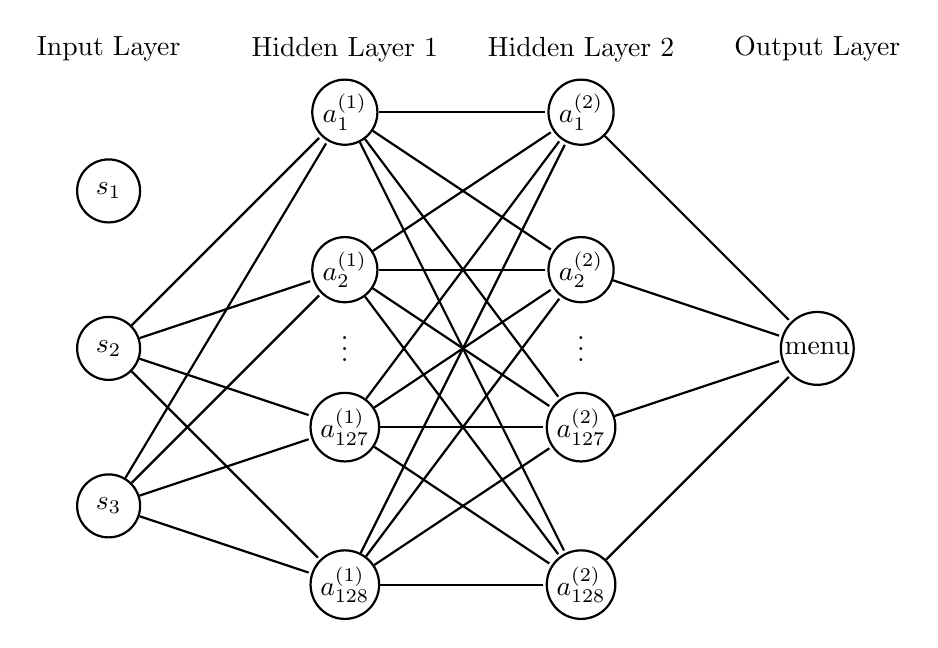
\begin{tikzpicture}[
    -,>=stealth',
    shorten >=1pt,
    auto,
    node distance=2cm,
    el/.style = {inner sep=2pt, align=left, sloped},
    thick,
    main node/.style={circle,fill=white!20,draw,minimum size=0.8cm, inner sep=1pt}
]

% Nodes
\node (l1) at (0, 3.8) {Input Layer};
\node[main node] at (0, 2) (s1) {$s_1$};
\node[main node] at (0, 0) (s2) {$s_2$};
\node[main node] at (0, -2) (s3) {$s_3$};
% \node[main node] at (0, -2.5) (s4) {$s_4$};

\node (l2) at (3, 3.8) {Hidden Layer 1};
\node[main node] at (3, 3) (a11) {$a_1^{(1)}$};
\node[main node] at (3, 1) (a12) {$a_2^{(1)}$};
% \node[main node] at (3, 1) (a13) {$a_3^{(1)}$};
% \node () at (3, 0) {$\cdots$};
% \node[main node] at (3, -1) (a16) {$a_{126}^{(1)}$};
\node () at (3, 0.1) {$\vdots$};
\node[main node] at (3, -1) (a17) {$a_{127}^{(1)}$};
\node[main node] at (3, -3) (a18) {$a_{128}^{(1)}$};

\node (l3) at (6, 3.8) {Hidden Layer 2};
\node[main node] at (6, 3) (a21) {$a_1^{(2)}$};
\node[main node] at (6, 1) (a22) {$a_2^{(2)}$};
% \node[main node] at (6, 1) (a23) {$a_3^{(2)}$};
% \node () at (6, 0) {$\cdots$};
% \node[main node] at (6, -1) (a26) {$a_{126}^{(2)}$};
\node () at (6, 0.1) {$\vdots$};
\node[main node] at (6, -1) (a27) {$a_{127}^{(2)}$};
\node[main node] at (6, -3) (a28) {$a_{128}^{(2)}$};

\node (l4) at (9, 3.8) {Output Layer};
\node [main node] (S) at (9,0) {menu};

% Edges between Input Layer and Hidden Layer 1
% \draw[] (s1) -- (a11);
% \draw[] (s1) -- (a12);
% \draw[] (s1) -- (a13);
% \draw[] (s1) -- (a16);
% \draw[] (s1) -- (a17);
% \draw[] (s1) -- (a18);

\draw[] (s2) -- (a11);
\draw[] (s2) -- (a12);
% \draw[] (s2) -- (a13);
% \draw[] (s2) -- (a16);
\draw[] (s2) -- (a17);
\draw[] (s2) -- (a18);

\draw[] (s3) -- (a11);
\draw[] (s3) -- (a12);
% \draw[] (s3) -- (a13);
% \draw[] (s3) -- (a16);
\draw[] (s3) -- (a17);
\draw[] (s3) -- (a18);

% \draw[] (s4) -- (a11);
% \draw[] (s4) -- (a12);
% \draw[] (s4) -- (a13);
% \draw[] (s4) -- (a16);
% \draw[] (s4) -- (a17);
% \draw[] (s4) -- (a18);

% Edges between Hidden Layer 1 and Hidden Layer 2
\draw[] (a11) -- (a21);
\draw[] (a11) -- (a22);
% \draw[] (a11) -- (a23);
% \draw[] (a11) -- (a26);
\draw[] (a11) -- (a27);
\draw[] (a11) -- (a28);

\draw[] (a12) -- (a21);
\draw[] (a12) -- (a22);
% \draw[] (a12) -- (a23);
% \draw[] (a12) -- (a26);
\draw[] (a12) -- (a27);
\draw[] (a12) -- (a28);

% \draw[] (a13) -- (a21);
% \draw[] (a13) -- (a22);
% \draw[] (a13) -- (a23);
% \draw[] (a13) -- (a26);
% \draw[] (a13) -- (a27);
% \draw[] (a13) -- (a28);

% \draw[] (a16) -- (a21);
% \draw[] (a16) -- (a22);
% \draw[] (a16) -- (a23);
% \draw[] (a16) -- (a26);
% \draw[] (a16) -- (a27);
% \draw[] (a16) -- (a28);

\draw[] (a17) -- (a21);
\draw[] (a17) -- (a22);
% \draw[] (a17) -- (a23);
% \draw[] (a17) -- (a26);
\draw[] (a17) -- (a27);
\draw[] (a17) -- (a28);

\draw[] (a18) -- (a21);
\draw[] (a18) -- (a22);
% \draw[] (a18) -- (a23);
% \draw[] (a18) -- (a26);
\draw[] (a18) -- (a27);
\draw[] (a18) -- (a28);

% Edges between Hidden Layer 2 and Output Layer
\draw[] (a21) -- (S);
\draw[] (a22) -- (S);
% \draw[] (a23) -- (S);
% \draw[] (a26) -- (S);
\draw[] (a27) -- (S);
\draw[] (a28) -- (S);

\end{tikzpicture}
}
\end{center}
\end{frame}

\begin{frame}{Objective / Loss function}
\begin{description}
    \item[Without fairness:] $C_1\cdot f(\nu(Y)) - B(Y)$ 
    \item[With fairness:]
$C_1\cdot f(\nu(Y)) - B(Y) + C_2\cdot Ev(Y)$, where $Ev(Y)$ is the number of student pairs $(s, s')$ where $s$ has justified envy toward $s'$ in $Y$. 
\end{description}
We choose $f(x)=x, C_1=4$, and $C_2=0.5$
\end{frame}

\section{Experiments}

\begin{frame}{Learning Settings}
\begin{itemize}
    \item 10 students, 6 colleges, the quota of each college is [2,2,1,2,1,2], there is one extra seat.
    \item The colleges' preferences are randomly generated (and fixed for the overall evaluation)
    \item 1 epoch contains: generating students' preferences, obtaining matchings, and applying feedback.
    \item 1,000 epoch for each trial. batch size: 32
\end{itemize}
    
\end{frame}

\begin{frame}{Comparison}
\centering
\begin{tabular}{crrr}
mechanism & average & envy & capacity \\ 
& Borda & violation & violation \\\hline
SD   & 4.7 & 1  & 0.0\\
ACDA  & 4.5 &  0.0 & 0.0\\
WO fairness  & 5.03 & 18.75 & 2.85 \\
% random preferences 5.16 19.7 2.7
% 全員同じpreferences 4.9 17.8 3.0
WT fairness  &  5.18 & 18.3 & 4.1 \\
% random preferences 5.06 23.6 3.2
% 全員同じpreferences 5.3 13.6 4.0
\end{tabular}
\end{frame}

\begin{frame}{Conclusions and Future works}
\begin{itemize}
    \item Although the Borda count is good (since quotas are expandable), the learned mechanism is not very good.
    \item The values of the loss function seem larger than the result of other mechanisms.
    \item Seems 1000 epochs is not enough?
    \item Need to try different network structures? 
    \item Need comparison with flexible DA. 
\end{itemize}    
\end{frame}
\begin{frame}{Another topic: Automated mechanism design using Constraint Satisfaction Problem (CSP)}
\begin{itemize}
\item There exists a set of $n$ variables $X$. 
Each variable $x_i$ takes its value from a discrete, finite domain $D_i$
\item Constraints are defined as nogoods. A nogood 
$((x_i, d_i), (x_j, d_j))$ means this combination is not allowed. 
\item The goal of a CSP is to find the value assignment of all variables that does not include any nogood. 
\item A Satisfiability Problem (SAT) is one kind of a canonical form of a CSP; any CSP can be converted into SAT automatically. 
\item Although CSP/SAT is NP-complete in general, there exist many open-source programs (SAT solvers) that can solve really huge SAT instances efficiently in practice (for a large problem instance, the main memory would be a bottle-neck). 
\end{itemize}
\end{frame}

\begin{frame}{Matching mechanism design as CSP}
\begin{itemize}
    \item Fix the number of students/colleges, colleges' preferences, and quotas, etc. 
\item Enumerate all possible students' preference profiles
\item For each profile, enumerate all matchings that satisfy desirable properties (except for strategy-proofness)
\item A profile is a variable, and its domain is the possible matchings
\item Enumerate all nogoods derived from strategy-proofness
\begin{itemize}
    \item Assume $\theta$ and $\theta'$, 
    which are different only for student $s$'s type.
    \item For $x\in D_{\theta}$ and $x'\in D_{\theta'}$, if $s$ prefers $x'$ over $x$, then 
    $((\theta, x), (\theta', x'))$ is a nogood. 
    \end{itemize}
\item If the obtained CSP is unsatisfiable, then no strategyproof mechanism exists. 
\item If it is satisfiable, the solution is a part of the mechanism 
(under the fixed colleges' preferences, etc.)
\end{itemize}
\end{frame}

\begin{frame}{Research Issue}
\begin{itemize}
    \item If the obtained CSP is unsatisfiable, we have an impossibility theorem (though making a human-readable proof is still an issue). 
    \item If the obtained CSP is satisfiable for several different settings, it is very likely a strategy-proof mechanism exists, but we just have many huge tables; we have no intuition how the mechanism looks like.
    \item Idea: can we use (deep) reinforcement learning to obtain rules that constitute the mechanism?  
\end{itemize}
\end{frame}

\begin{frame}{Applying reinforcement learning}
\begin{itemize}
    \item Assume a state (in the reinforcement learning) is represented as a students' preference profile, a partial matching, and \emph{forbidden pairs}.
    \item A forbidden pair $(s,c)$ is a pair of student $s$ and college $c$, which means that $s$ cannot be accepted to college $c$.
    \item In a given state, if all students can be accepted to her first-choice college (which is not forbidden), we assume it is a terminal state.
    \item Otherwise, the mechanism takes an action, which is either (i) a particular pair $(s,c)$ is forbidden, or (ii) a particular pair $(s,c)$ is added to the partial matching; then a new state is obtained. 
    \item By reaching a correct (or wrong) terminal state (which is defined by the CSP solution, some positive (or negative) reward is given.  
    \item After the learning process converges, we know the correct action for each state, which gives us a more detailed description of the mechanism obtained by CSP. 
\end{itemize}
    
\end{frame}

\begin{frame}
\frametitle{References}
\note{Thank you for listening.}



\small
\bibliographystyle{plainnat}
\bibliography{reference,thesis}

\end{frame}
\end{document}

